% =============================================================================
% main.tex — document maître
% Compilation : voir README.md à la racine du dossier rapport_latex/
% =============================================================================
\documentclass[12pt,a4paper]{report}

% =============================================================================
% preambule.tex — packages et réglages de mise en forme (normes PFE marocaines)
% =============================================================================

% --- Langue ---
\usepackage[french]{babel}
\usepackage[T1]{fontenc}
\usepackage[utf8]{inputenc}

% --- Police : rendu proche Times New Roman ---
\usepackage{mathptmx}

% --- Interligne 1,5 ---
\usepackage{setspace}
\onehalfspacing

% --- Marges 2,5 cm ---
\usepackage[margin=2.5cm]{geometry}

% --- Figures / tableaux ---
\usepackage{graphicx}
\graphicspath{{images/}{../diagrammes/images/}}
\usepackage{float}                 % positionnement stable avec [H]
\usepackage{rotating}              % figures en paysage (sidewaysfigure) pour les diagrammes très larges
\usepackage{caption}
\captionsetup[table]{position=above}   % légendes tableaux au-dessus
\captionsetup[figure]{position=below}  % légendes figures en dessous (par défaut, explicite ici)

% Numérotation des figures et tableaux par chapitre → Figure 2.1, Tableau 3.2
\counterwithin{figure}{chapter}
\counterwithin{table}{chapter}

% --- Tableaux enrichis ---
\usepackage{booktabs}
\usepackage{longtable}
\usepackage{array}

% --- Extraits de code (Java / PlantUML) ---
\usepackage{xcolor}
\usepackage{listings}
\definecolor{codegray}{rgb}{0.95,0.95,0.95}
\definecolor{codekeyword}{rgb}{0.0,0.0,0.6}
\definecolor{codecomment}{rgb}{0.35,0.55,0.35}
\lstdefinestyle{javastyle}{
  backgroundcolor=\color{codegray},
  basicstyle=\ttfamily\footnotesize,
  keywordstyle=\color{codekeyword}\bfseries,
  commentstyle=\color{codecomment}\itshape,
  numbers=left,
  numberstyle=\tiny,
  frame=single,
  breaklines=true,
  showstringspaces=false,
  language=Java,
  captionpos=b,
}
\lstset{style=javastyle}

% --- Liens cliquables (table des matières, \ref, bibliographie) ---
\usepackage{hyperref}
\hypersetup{
  colorlinks=true,
  linkcolor=black,
  citecolor=black,
  urlcolor=blue,
  pdftitle={Rapport de Projet de Fin d'Études — IAT Academy},
}

% --- Bibliographie ---
% Style ieee par défaut (adapté à un rapport d'ingénierie logicielle) ;
% remplacer par style=apa si l'établissement l'exige.
\usepackage[backend=biber,style=ieee,sorting=none]{biblatex}
\addbibresource{bibliographie.bib}

% --- Divers ---
\usepackage{enumitem}
\usepackage{textcomp}
\usepackage{csquotes}


\begin{document}

% -----------------------------------------------------------------------------
% Pages liminaires — pagination romaine
% -----------------------------------------------------------------------------
\pagenumbering{roman}

% =============================================================================
% page_de_garde.tex — personnalisez les champs ci-dessous (établissement,
% filière, noms, encadrants, année universitaire).
% =============================================================================

\begin{titlepage}
  \centering

  % --- Logo établissement (remplacez par le vôtre dans rapport_latex/images/) ---
  
\includegraphics[width=3.5cm]{logo_ecole_placeholder.png} % TODO: remplacez ce fichier

  \vspace{0.5cm}
  {\large \MakeUppercase{[Nom de l'établissement]} \par}
  {\normalsize [Filière — ex. Génie Informatique / Ingénierie Logicielle] \par}

  \vspace{2cm}
  \rule{0.9\textwidth}{1pt}\par
  \vspace{0.4cm}
  {\Huge\bfseries Rapport de Projet de Fin d'Études \par}
  \vspace{0.4cm}
  \rule{0.9\textwidth}{1pt}\par

  \vspace{1cm}
  {\LARGE \bfseries IAT Academy \par}
  {\large Conception et réalisation d'une plateforme e-learning pour les métiers \\
   de l'aviation, de l'accueil et du tourisme \par}

  \vspace{2cm}
  
\includegraphics[width=2.6cm]{logo_iat.png}

  \vspace{2cm}
  \begin{minipage}[t]{0.45\textwidth}
    \begin{flushleft} \large
      \textbf{Réalisé par :} \\{}
      [Prénom NOM]
    \end{flushleft}
  \end{minipage}
  \hfill
  \begin{minipage}[t]{0.45\textwidth}
    \begin{flushright} \large
      \textbf{Encadré par :} \\{}
      [Encadrant académique — Prénom NOM] \\{}
      [Encadrant professionnel — Prénom NOM]
    \end{flushright}
  \end{minipage}

  \vfill
  {\large Année universitaire [2025 -- 2026] \par}

\end{titlepage}


\chapter*{Remerciements}
Je tiens à exprimer ma sincère gratitude à mon encadrant académique pour
son suivi attentif tout au long de ce projet, sa disponibilité et la
pertinence de ses remarques, qui ont considérablement enrichi la démarche
suivie dans ce travail. Mes remerciements vont également à mon encadrant
professionnel au sein d'IAT Academy, pour la confiance qu'il m'a accordée
dès le début du stage en me confiant un périmètre technique aussi complet,
et pour le temps consacré à clarifier les règles métier propres au cursus
de l'académie --- sans lesquelles la conception du système de progression
par unité de formation n'aurait pas pu aboutir à une solution fidèle à la
réalité du terrain.

Je remercie chaleureusement l'ensemble de l'équipe pédagogique et
administrative d'IAT Academy pour son accueil, sa bienveillance et sa
disponibilité à répondre à mes questions tout au long de l'immersion dans
le fonctionnement de l'académie. Cette collaboration au quotidien a été
déterminante pour comprendre non seulement les besoins fonctionnels
exprimés, mais aussi les contraintes réelles d'exploitation d'une
plateforme destinée à des apprenants et des formateurs aux profils variés.

Je souhaite également remercier le corps professoral de mon établissement
pour la formation théorique et pratique reçue tout au long de mon cursus,
qui a constitué le socle indispensable à la réalisation de ce projet, ainsi
que les membres du jury pour l'intérêt qu'ils porteront à ce travail.

Enfin, mes remerciements les plus personnels vont à ma famille et à mes
proches, pour leur soutien constant et leurs encouragements tout au long de
cette période de stage.

\chapter*{Résumé}
IAT Academy est une plateforme e-learning destinée aux métiers de l'aviation, de
l'accueil et du tourisme, développée avec Spring Boot (backend) et Next.js
(frontend). Ce rapport présente le contexte du projet, l'analyse et la
conception de la solution, les choix techniques réalisés lors de l'implémentation
— en particulier les mécanismes qui dépassent le simple CRUD (correction de
quiz, génération de questions par intelligence artificielle, contrôle d'accès à
granularité fine, etc. — voir chapitre 3) — ainsi que la démarche de tests et de
déploiement.

\textbf{Mots-clés :} e-learning, Spring Boot, Spring Security, PostgreSQL,
Redis, intelligence artificielle, architecture en couches.

\chapter*{Abstract}
IAT Academy is an e-learning platform for aviation, hospitality and tourism
training programs, built with Spring Boot (backend) and Next.js (frontend).
This report presents the project context, the analysis and design of the
solution, the technical decisions made during implementation — particularly the
mechanisms that go beyond simple CRUD (quiz grading, AI-assisted question
generation, fine-grained access control, etc. — see Chapter 3) — and the
testing and deployment approach.

\textbf{Keywords:} e-learning, Spring Boot, Spring Security, PostgreSQL, Redis,
artificial intelligence, layered architecture.

\tableofcontents
\listoffigures
\listoftables

% -----------------------------------------------------------------------------
% Corps du rapport — pagination arabe à partir de l'introduction
% -----------------------------------------------------------------------------
\cleardoublepage
\pagenumbering{arabic}

\chapter*{Introduction générale}
\addcontentsline{toc}{chapter}{Introduction générale}

La transformation numérique des organismes de formation professionnelle ne
se limite plus, aujourd'hui, à la simple mise en ligne de supports de
cours. Elle touche l'ensemble du cycle de vie de l'apprenant : son
inscription, le suivi minutieux de sa progression, l'évaluation de ses
compétences par des modalités variées, l'accompagnement individualisé
jusqu'à l'obtention d'un diplôme, et jusqu'à la valorisation de ce diplôme
sur le marché de l'emploi. C'est dans ce contexte qu'a été pensé et
développé IAT Academy, une plateforme e-learning destinée à un cycle
professionnel de deux années dans les métiers de l'aviation, de l'accueil
et du tourisme --- des filières où l'employabilité concrète des diplômés
constitue l'indicateur de réussite ultime, bien plus qu'un simple taux de
réussite académique.

Avant ce projet, la gestion pédagogique d'IAT Academy s'appuyait sur des
outils et des supports dispersés, sans espace numérique centralisé
permettant de suivre en temps réel la progression d'un apprenant à travers
les différentes unités de formation qui composent son cursus, ni de
garantir que les étapes-clés du parcours --- en particulier celles qui
exigent un jugement humain, comme la validation du stage en entreprise ---
soient réellement respectées avant qu'un module supérieur ne devienne
accessible. La problématique centrale de ce projet peut donc se formuler
ainsi : \emph{comment concevoir et développer une plateforme qui structure,
sécurise et automatise l'intégralité du parcours pédagogique d'un
apprenant, de la candidature à la délivrance d'un certificat vérifiable,
tout en respectant des règles métier qui ne se réduisent jamais à un simple
calcul automatique de score ?}

Pour répondre à cette problématique, ce stage de fin d'études a consisté à
concevoir et implémenter, de bout en bout, une application composée d'un
backend Spring Boot exposant une API REST sécurisée et d'un frontend
Next.js consommant cette API. Le travail réalisé couvre l'ensemble des
étapes d'un projet logiciel réel : l'analyse des besoins et la
modélisation du domaine métier, la conception d'une architecture en
couches capable de supporter des règles de progression complexes, la mise
en \oe uvre de mécanismes qui dépassent largement le simple CRUD ---
notamment une intégration à des services d'intelligence artificielle
générative pour assister la création de contenu pédagogique --- ainsi que
la validation de l'ensemble par une suite de tests automatisés et une
démarche de déploiement conteneurisé.

Ce rapport est organisé en quatre chapitres. Le premier chapitre présente
le contexte général du projet : l'organisme d'accueil, la problématique
métier identifiée et les objectifs poursuivis. Le deuxième chapitre détaille
l'analyse des besoins et les choix de conception qui en découlent ---
acteurs, cas d'utilisation, modèle de données et architecture logicielle.
Le troisième chapitre, cœur technique de ce rapport, présente
l'implémentation réalisée en mettant l'accent sur les mécanismes qui
constituent la véritable valeur ajoutée du projet, classés par ordre
d'impact et systématiquement rattachés au code source qui les concrétise.
Le quatrième et dernier chapitre décrit la démarche de validation par les
tests et l'architecture de déploiement retenue. Une conclusion générale
revient enfin sur les apports de ce travail et ouvre sur ses perspectives
d'évolution.

\chapter{Contexte général du projet}
\label{ch:contexte}

\section{Organisme d'accueil}

IAT Academy est une académie de formation professionnelle spécialisée dans
les métiers de l'aviation, de l'accueil et du tourisme, préparant en
particulier aux filières Hôtesse de l'air et Steward, Agent d'escale,
Accompagnateur touristique, et Réception hôtelière. La formation se
déroule sur un cycle professionnel de deux années, structuré autour d'un
équilibre volontairement assumé entre théorie et pratique : cours en
présentiel dispensés par des formateurs issus directement du secteur
(compagnies aériennes, groupes hôteliers, agences de voyage), stage en
milieu réel intégré au cursus plutôt que relégué à une simple option de
fin de parcours, et, désormais, un espace d'apprentissage numérique
prolongeant la salle de classe au-delà des heures de cours.

Cette double identité --- académie de formation aux métiers du transport
aérien et du tourisme, mais aussi organisme dont l'indicateur de réussite
premier reste l'insertion professionnelle effective de ses diplômés ---
irrigue l'ensemble des choix fonctionnels du projet. Elle explique
pourquoi le référentiel de compétences se traduit directement dans
l'organisation du contenu pédagogique (unités de formation alignées sur
les compétences métier attendues par les employeurs du secteur), pourquoi
le stage occupe une place aussi centrale dans le modèle de progression
(voir chapitre~\ref{ch:analyse-conception}), et pourquoi la plateforme
intègre jusqu'à un mécanisme de certification vérifiable publiquement et
de partage professionnel sur les réseaux sociaux (voir
chapitre~\ref{ch:realisation}) --- un choix qui, sur un plan strictement
académique, pourrait sembler périphérique, mais qui prend tout son sens
dès lors que l'on considère la mission réelle de l'académie : préparer ses
apprenants non pas seulement à réussir des examens, mais à être recrutés.
L'identité visuelle de la plateforme reprend d'ailleurs ce parti pris
métier jusque dans son vocabulaire d'interface, construit autour de la
métaphore de la carte d'embarquement --- un choix esthétique qui ancre
délibérément l'expérience numérique dans l'univers professionnel visé par
les apprenants.

\section{Contexte et problématique}

Avant ce projet, le suivi pédagogique d'IAT Academy reposait sur des
supports et des outils non centralisés : le contenu de cours, l'évaluation
des apprenants et le suivi de leur progression n'étaient réunis dans aucun
espace numérique unique. Cette situation, courante dans de nombreux
établissements de formation professionnelle de taille intermédiaire,
posait en pratique plusieurs difficultés concrètes que ce projet s'est
attaché à résoudre une à une.

La première difficulté tenait à l'absence de toute vue d'ensemble, en
temps réel, de la progression d'un apprenant à travers les deux années de
son cursus. Sans outil centralisé, savoir précisément où en est un
apprenant donné --- quels modules il a complétés, quelles évaluations lui
restent à passer, si son stage a été validé --- exigeait de recouper
manuellement plusieurs sources d'information, un exercice difficilement
soutenable à l'échelle de plusieurs promotions. La seconde difficulté
concernait l'évaluation elle-même : les quiz, devoirs et réponses libres
des apprenants n'étaient ni centralisés, ni tracés de façon homogène,
rendant la correction et le suivi des notes dépendants de pratiques
individuelles plutôt que d'un processus outillé et cohérent.

La troisième difficulté, sans doute la plus structurante pour la
conception technique du projet, était l'absence de tout mécanisme fiable
de validation d'étape : rien, dans l'organisation existante, n'empêchait
techniquement un apprenant d'accéder à du contenu avancé sans avoir
réellement validé les prérequis correspondants --- une lacune d'autant
plus problématique que certaines étapes du cursus d'IAT Academy, comme la
validation du stage en entreprise ou de la soutenance finale, ne peuvent
pas se réduire à un critère automatique et exigent le jugement explicite
du Directeur pédagogique. Enfin, la délivrance et la vérification des
certificats de réussite reposaient sur un processus entièrement manuel,
sans preuve numérique qu'un tiers extérieur --- un employeur, un
partenaire du secteur --- puisse vérifier de façon autonome.

Cette analyse conduit à formuler la problématique centrale de ce projet de
la manière suivante : \emph{comment structurer, sécuriser et automatiser
le parcours pédagogique complet d'un apprenant --- de l'inscription à la
délivrance du certificat --- tout en respectant des règles métier qui ne
se réduisent jamais à de simples critères automatiques, puisque certaines
étapes-clés exigent explicitement l'implication du Directeur
pédagogique ?} C'est cette tension entre automatisation et jugement
humain, plus que la seule numérisation d'un contenu de cours, qui a guidé
l'ensemble des choix de conception présentés au
chapitre~\ref{ch:analyse-conception}.

\section{Objectifs du projet}

Pour répondre à cette problématique, six objectifs concrets ont structuré
le travail réalisé durant ce stage.

Le premier objectif consistait à concevoir un modèle de données
représentant fidèlement la structure pédagogique réelle du cursus ---
Formation, Année, Unité de Formation, Module, Leçon, puis Bloc de contenu
--- sans pour autant complexifier inutilement le schéma relationnel sous-jacent ;
ce choix de modélisation, en apparence anodin, s'est révélé être l'une des
décisions de conception les plus structurantes du projet, comme le détaille
la section~\ref{sec:analyse-conception} du chapitre suivant. Le deuxième
objectif visait à mettre en place un système d'évaluation complet, capable
de gérer plusieurs types de quiz selon leur portée --- section, module, fin
d'unité de formation, fin d'année --- ainsi que plusieurs types de
questions, avec à la fois une correction automatique pour les questions à
choix et une correction manuelle pour les réponses libres, ces deux modes
devant in fine converger vers un seul et même score final cohérent.

Le troisième objectif était de garantir un déblocage séquentiel du contenu
pédagogique fondé sur des règles vérifiées côté serveur, et non pas
seulement suggérées côté interface --- une exigence de sécurité autant que
de fiabilité pédagogique. Le quatrième objectif consistait à fournir à
l'équipe pédagogique d'IAT Academy un espace d'administration complet,
lui permettant de produire le contenu de cours, de corriger les
évaluations, de suivre individuellement chaque apprenant et de réaliser les
validations manuelles qui, comme évoqué plus haut, ne peuvent être
déléguées à un algorithme. Le cinquième objectif visait à automatiser la
délivrance de certificats numériquement vérifiables, tout en outillant le
suivi du stage jusqu'à sa signature par un tuteur externe à l'académie.
Enfin, le sixième objectif portait sur la sécurisation transversale de
l'ensemble de la plateforme --- authentification, séparation stricte des
rôles, protection contre les abus des fonctionnalités exposées à des
services tiers --- et sur son déploiement de façon reproductible, condition
nécessaire à une exploitation réelle au-delà du cadre du stage.

\section{Méthodologie de travail et planning}

Le développement du projet a suivi une démarche itérative, par
fonctionnalité plutôt que par couche technique : chaque bloc fonctionnel
--- authentification, catalogue de cours, système de quiz, gestion du
stage, certification, puis les fonctionnalités transverses de
communication et de sécurité --- a été conçu, implémenté et testé de bout
en bout (du modèle de données jusqu'à l'interface) avant de passer au
suivant, plutôt que de développer séparément l'intégralité du backend puis
l'intégralité du frontend. Cette approche a permis de valider très tôt,
sur des cas concrets, que le modèle de données retenu tenait effectivement
la charge des règles métier réelles --- en particulier la logique de
progression par unité de formation --- avant d'investir du temps de
développement sur les fonctionnalités qui en dépendent.

Des points d'avancement réguliers avec l'encadrant professionnel au sein
d'IAT Academy ont permis de confronter les choix techniques aux
contraintes réelles de l'académie, notamment sur les points où une règle
métier n'était pas immédiatement évidente à traduire en logique
applicative --- la distinction entre les unités de formation exigeant une
validation manuelle du Directeur et celles n'en exigeant pas en est
l'exemple le plus révélateur (voir section~\ref{sec:progression-uf}).

Le temps du stage s'est réparti, dans ses grandes masses, entre une phase
initiale de cadrage et d'analyse des besoins auprès de l'équipe
pédagogique, une phase de conception du modèle de données et de
l'architecture --- la plus déterminante pour la suite, dans la mesure où
une erreur de modélisation à ce stade se serait répercutée sur l'ensemble
du développement ---, une phase de développement à proprement parler,
volontairement la plus longue, menée fonctionnalité par fonctionnalité
comme décrit ci-dessus, et enfin une phase de consolidation regroupant les
tests, la correction des anomalies détectées et la rédaction du présent
rapport. Le tableau~\ref{tab:planning} synthétise cette répartition ; il
peut être complété par un diagramme de Gantt détaillé si le format attendu
par l'établissement l'exige.

\begin{table}[H]
  \centering
  \caption{Répartition indicative des grandes phases du projet}
  \label{tab:planning}
  \begin{tabular}{@{}p{5cm}p{8cm}@{}}
    \toprule
    Phase & Contenu principal \\
    \midrule
    Cadrage et analyse des besoins & Immersion dans le fonctionnement d'IAT Academy, recueil des règles métier, définition du périmètre. \\
    Conception & Modélisation des entités, choix d'architecture, définition des mécanismes de sécurité. \\
    Développement & Implémentation backend et frontend, fonctionnalité par fonctionnalité. \\
    Consolidation & Rédaction et exécution des tests, correction des anomalies, rédaction du rapport. \\
    \bottomrule
  \end{tabular}
\end{table}

\section{Conclusion}

Ce chapitre a présenté le contexte métier d'IAT Academy, la problématique
qui a motivé ce projet --- automatiser un parcours pédagogique complexe
sans sacrifier les validations qui exigent un jugement humain --- ainsi
que les objectifs et la méthodologie qui en découlent. Le
chapitre~\ref{ch:analyse-conception} détaille maintenant l'analyse
fonctionnelle et les choix de conception qui répondent concrètement à ces
objectifs.

\chapter{Analyse et conception}
\label{ch:analyse-conception}

\section{Acteurs et cas d'utilisation}

Le système distingue cinq rôles internes, organisés en une hiérarchie de
sécurité (\texttt{ROLE\_SUPER\_ADMIN > ROLE\_ADMIN}), à laquelle s'ajoutent
deux acteurs externes ne possédant pas de compte : le tuteur de stage
(accès par lien à usage unique) et le visiteur public (formulaire de
contact, infolettre, vérification de certificat).

\begin{table}[H]
  \centering
  \caption{Rôles applicatifs et responsabilités}
  \label{tab:roles}
  \begin{tabular}{@{}p{2.8cm}p{9.5cm}@{}}
    \toprule
    Rôle & Responsabilités \\
    \midrule
    \texttt{SUPER\_ADMIN} & Paramètres système globaux, en plus de tous les droits Admin. \\
    \texttt{ADMIN} (Directeur) & Gestion pédagogique complète, validation des UF sensibles, gestion des groupes et des campagnes email, en plus de tous les droits Formateur. \\
    \texttt{FORMATEUR} & Studio de cours, gestion des quiz, correction manuelle, messagerie, bourse à l'emploi. \\
    \texttt{ETUDIANT} & Espace apprenant : contenu, quiz, stage, certificat, messagerie. \\
    \texttt{SUPPORT} & Accès limité, essentiellement en lecture. \\
    \bottomrule
  \end{tabular}
\end{table}

La Figure~\ref{fig:cas-utilisation} synthétise l'ensemble des cas
d'utilisation identifiés à partir des 29 contrôleurs REST exposés par le
backend.

\begin{figure}[H]
  \centering
  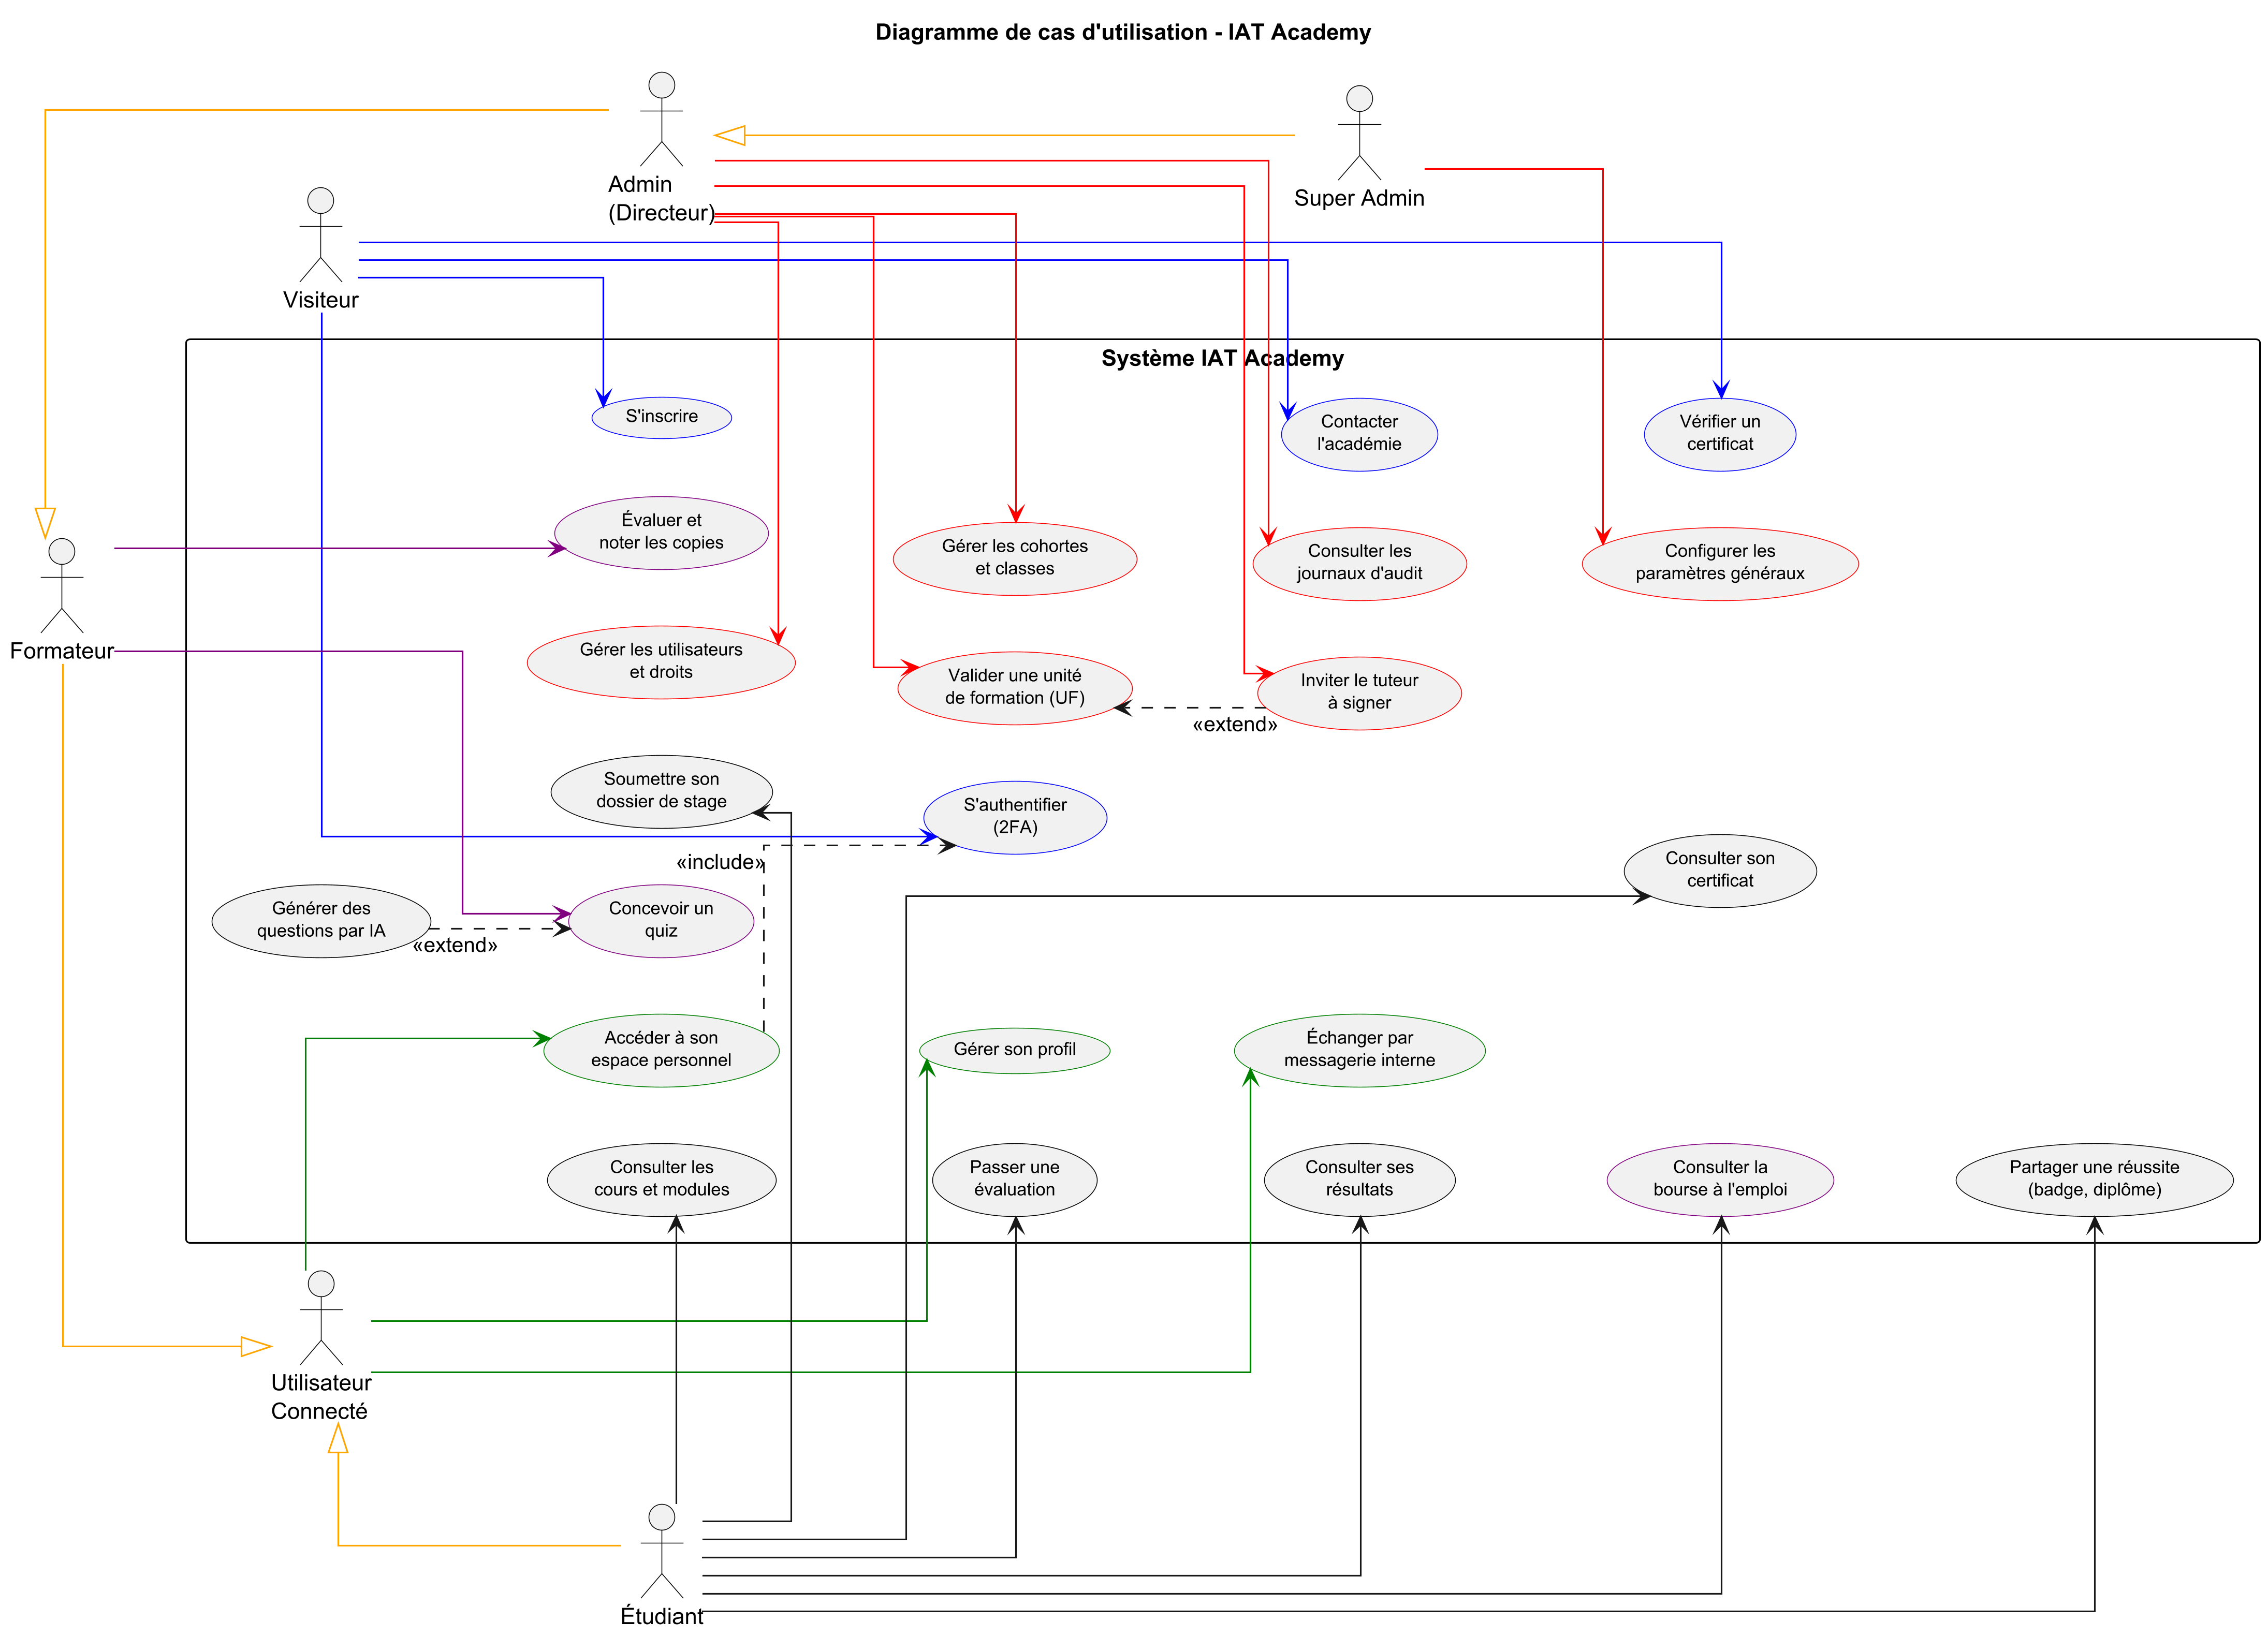
\includegraphics[width=\textwidth,height=0.85\textheight,keepaspectratio]{diagramme_cas_utilisation.png}
  \caption{Diagramme de cas d'utilisation}
  \label{fig:cas-utilisation}
\end{figure}

\section{Modèle de données}
\label{sec:analyse-conception}

Le modèle de données regroupe 39 entités JPA concrètes, toutes héritant
--- à l'exception d'\texttt{AssetDownload} --- d'une superclasse technique
abstraite \texttt{AuditableEntity} (\texttt{createdAt}/\texttt{updatedAt}).
La Figure~\ref{fig:classes-ensemble}
en donne une vue d'ensemble au format UML standard, organisée en huit
paquetages fonctionnels avec leurs attributs principaux, leurs
associations et les cardinalités correspondantes. Trois domaines jugés
les plus structurants pour la compréhension du système sont ensuite
détaillés à un niveau plus fin : structure pédagogique et groupes
(Figure~\ref{fig:classes-pedagogie}), évaluation
(Figure~\ref{fig:classes-evaluation}), et stage et certification
(Figure~\ref{fig:classes-stage}). Les domaines restants (communication,
marketing/emploi, médias, suivi système) suivent les mêmes conventions de
modélisation et sont détaillés au besoin dans le code source
(\texttt{domain/entity/}).

\begin{sidewaysfigure}
  \centering
  \includegraphics[width=\textwidth,height=0.9\textheight,keepaspectratio]{diagramme_classes_ensemble.png}
  \caption{Diagramme de classes — vue d'ensemble de l'application}
  \label{fig:classes-ensemble}
\end{sidewaysfigure}

\begin{figure}[H]
  \centering
  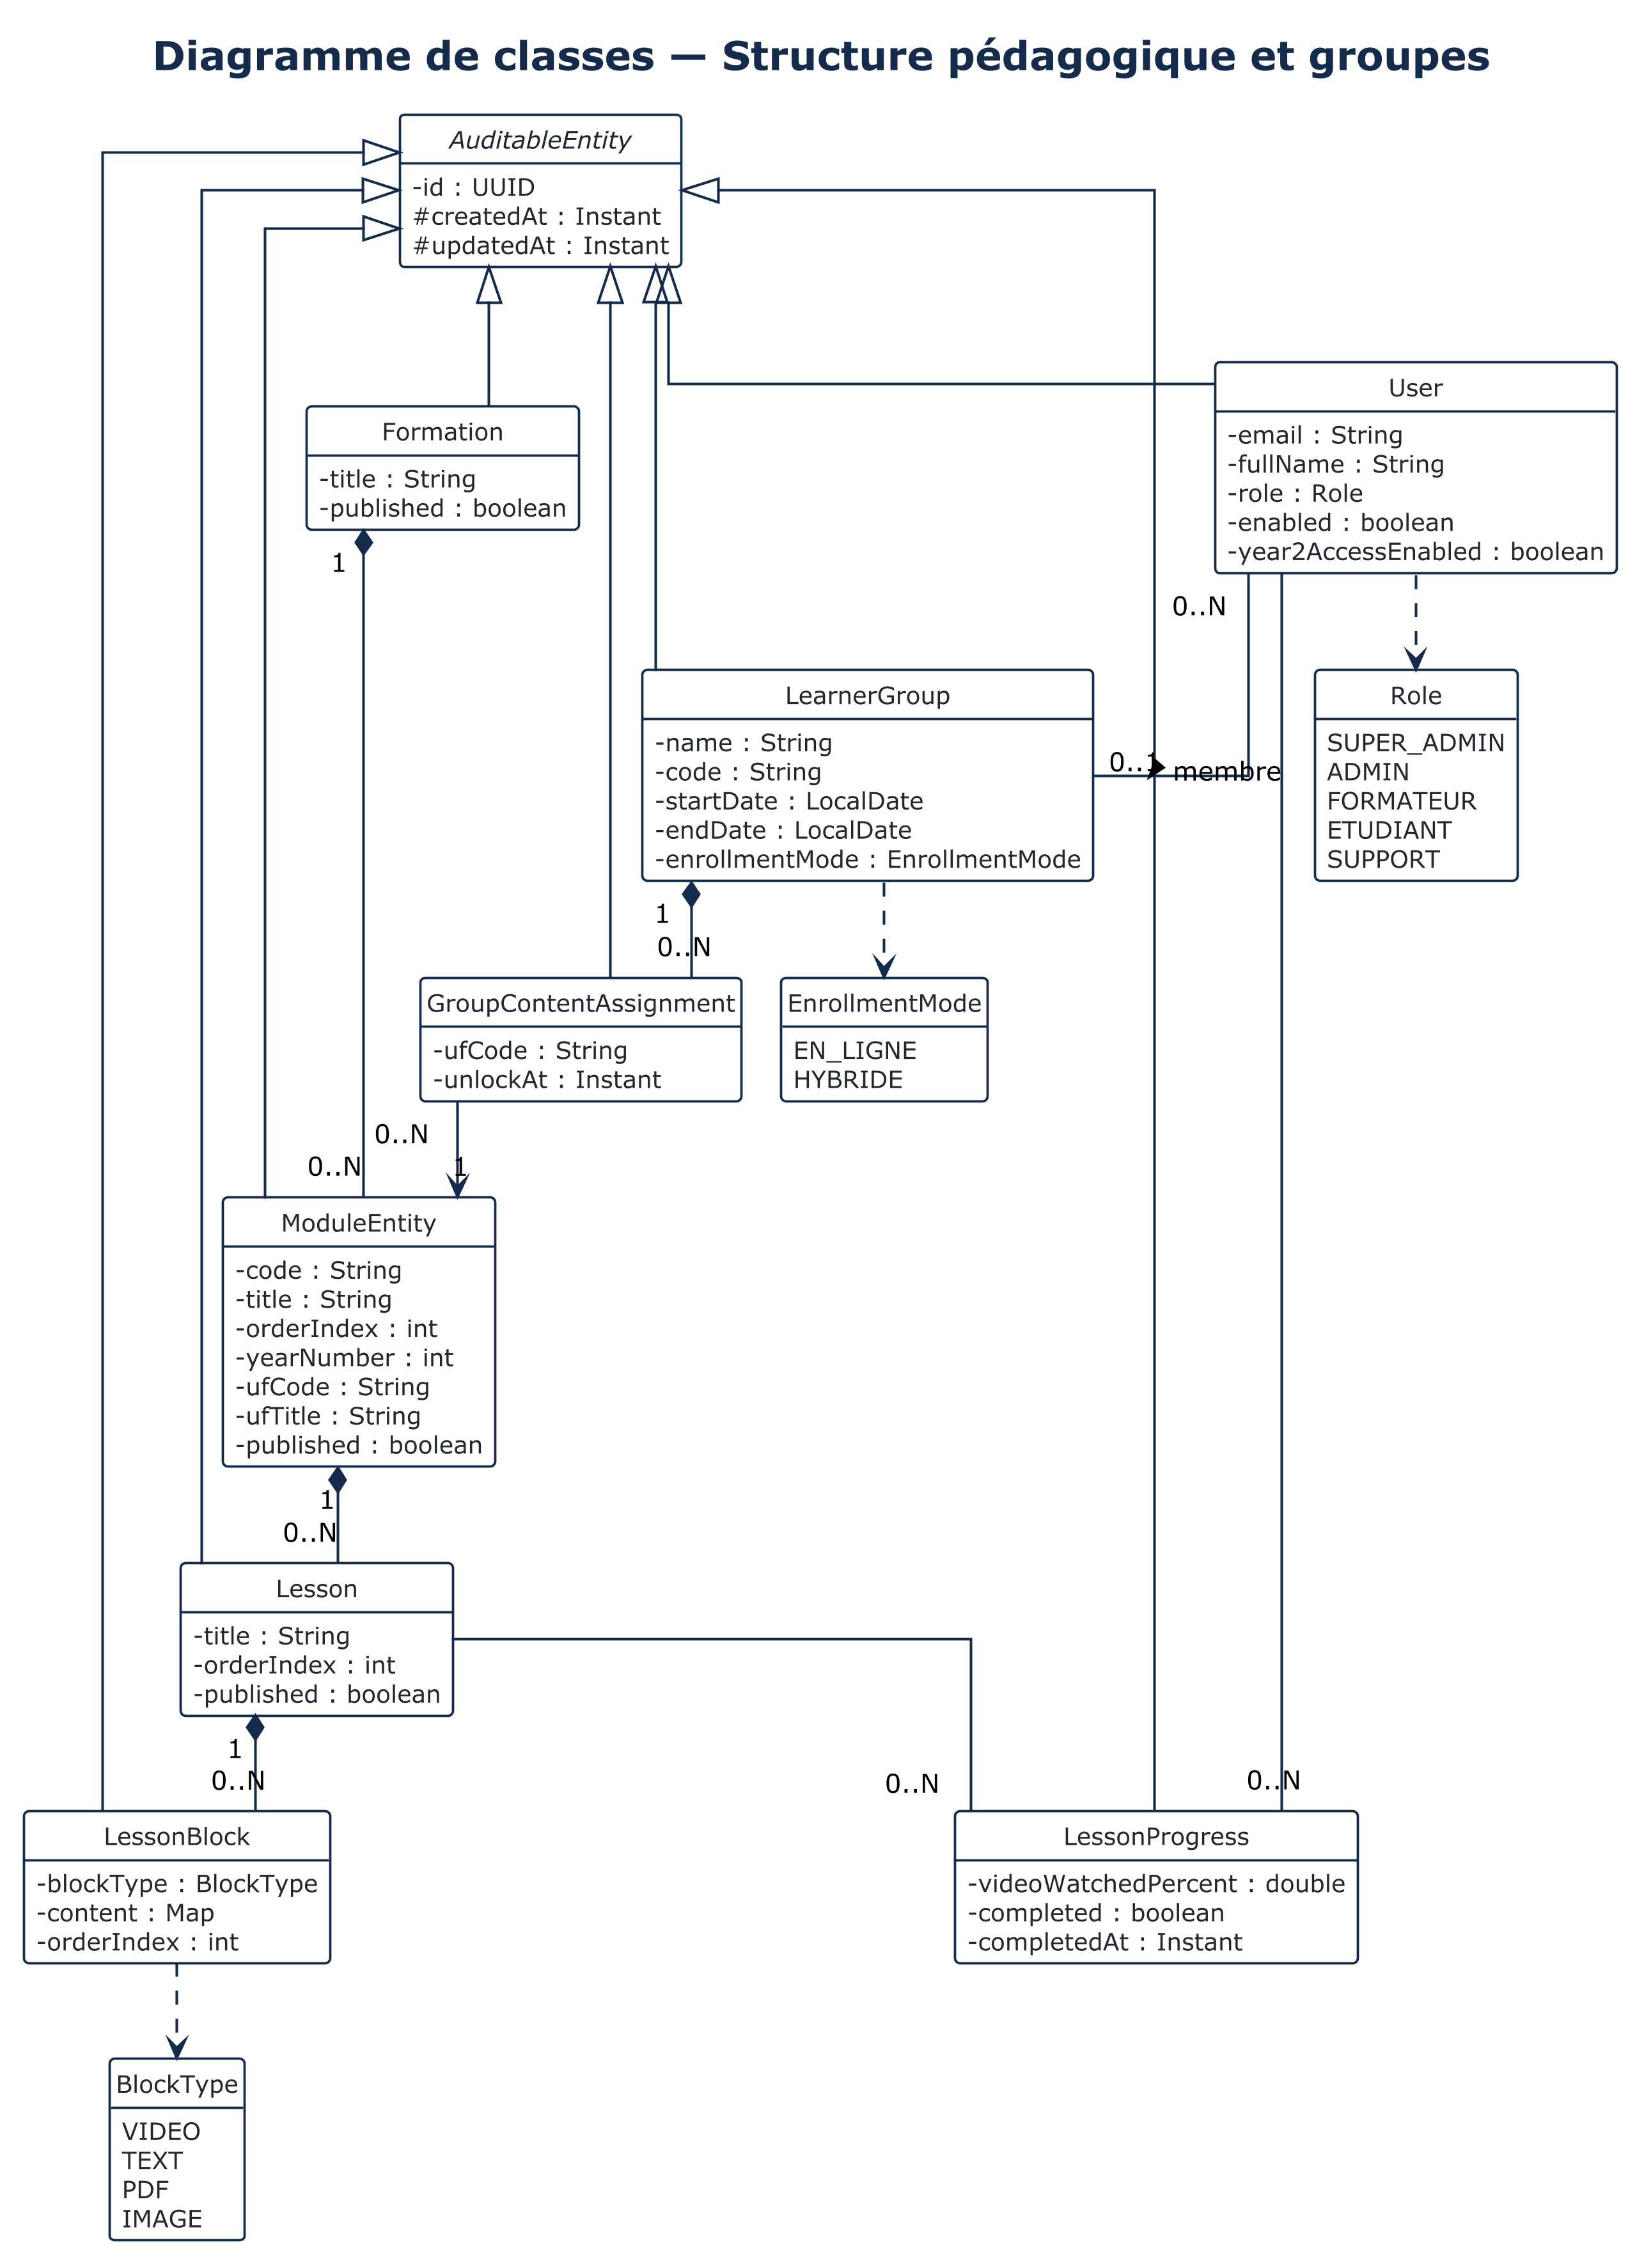
\includegraphics[width=\textwidth,height=0.85\textheight,keepaspectratio]{diagramme_classes_pedagogie.png}
  \caption{Diagramme de classes — structure pédagogique et groupes}
  \label{fig:classes-pedagogie}
\end{figure}

\begin{figure}[H]
  \centering
  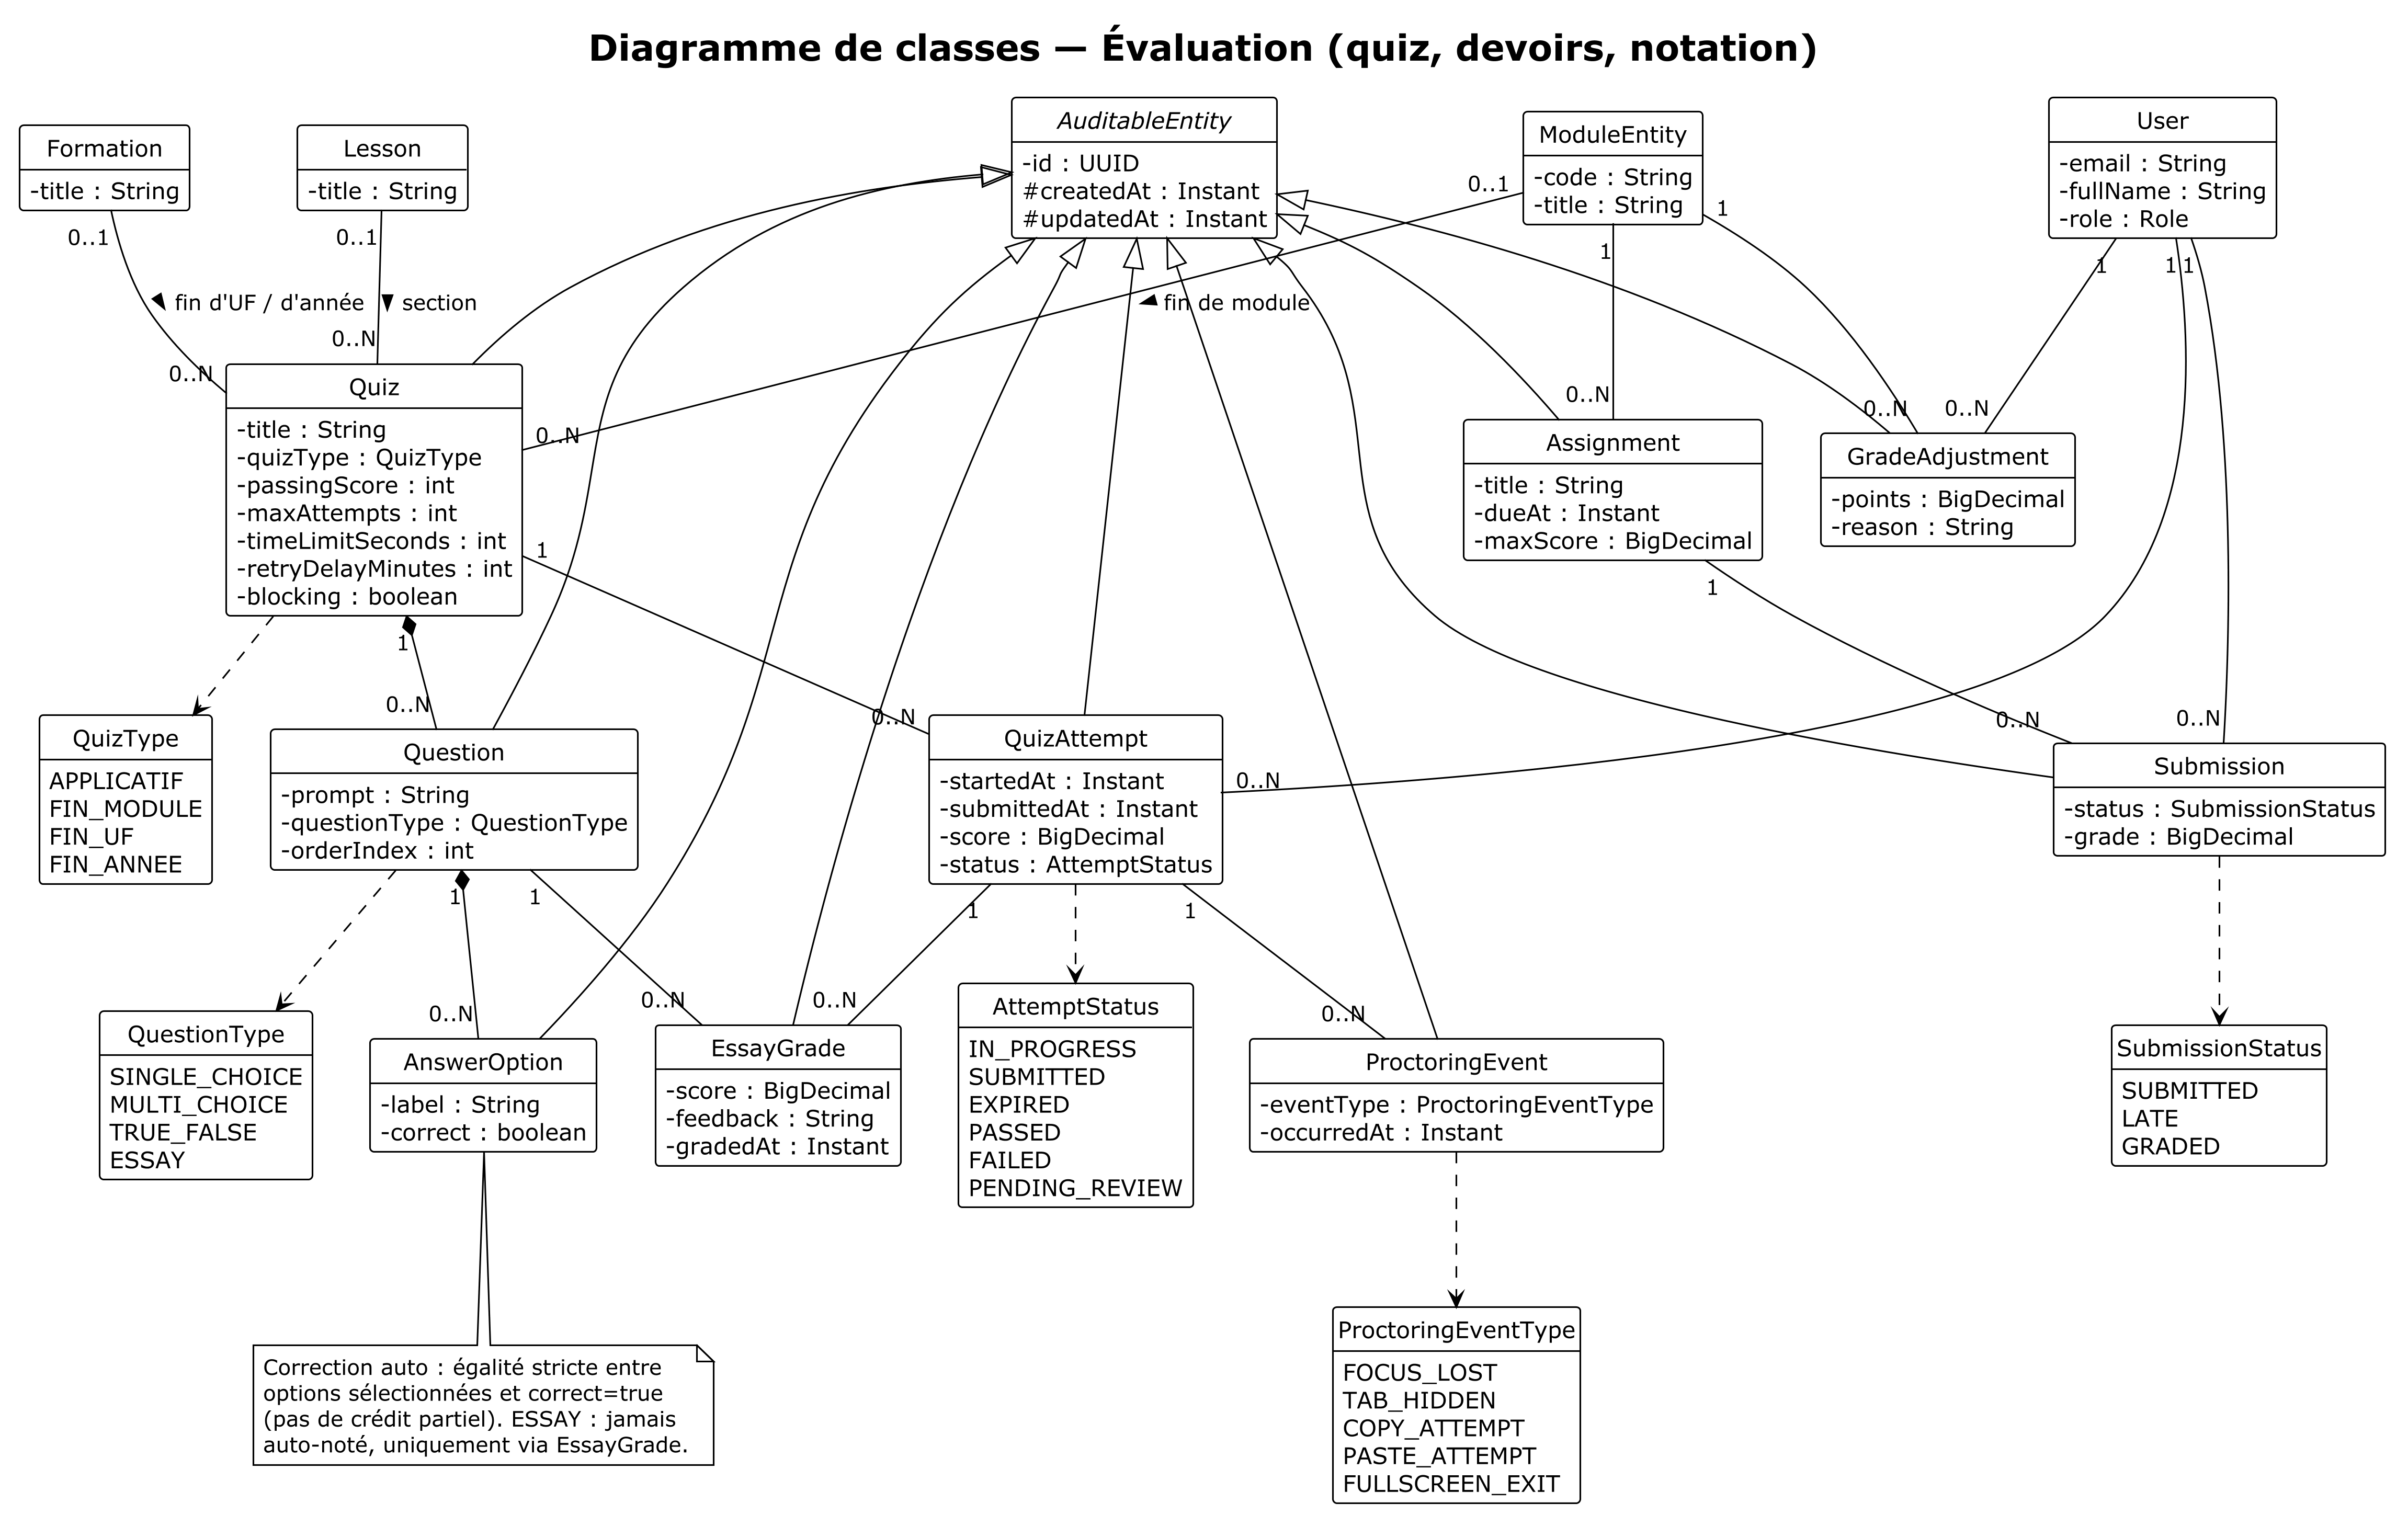
\includegraphics[width=\textwidth,height=0.85\textheight,keepaspectratio]{diagramme_classes_evaluation.png}
  \caption{Diagramme de classes — évaluation}
  \label{fig:classes-evaluation}
\end{figure}

\begin{figure}[H]
  \centering
  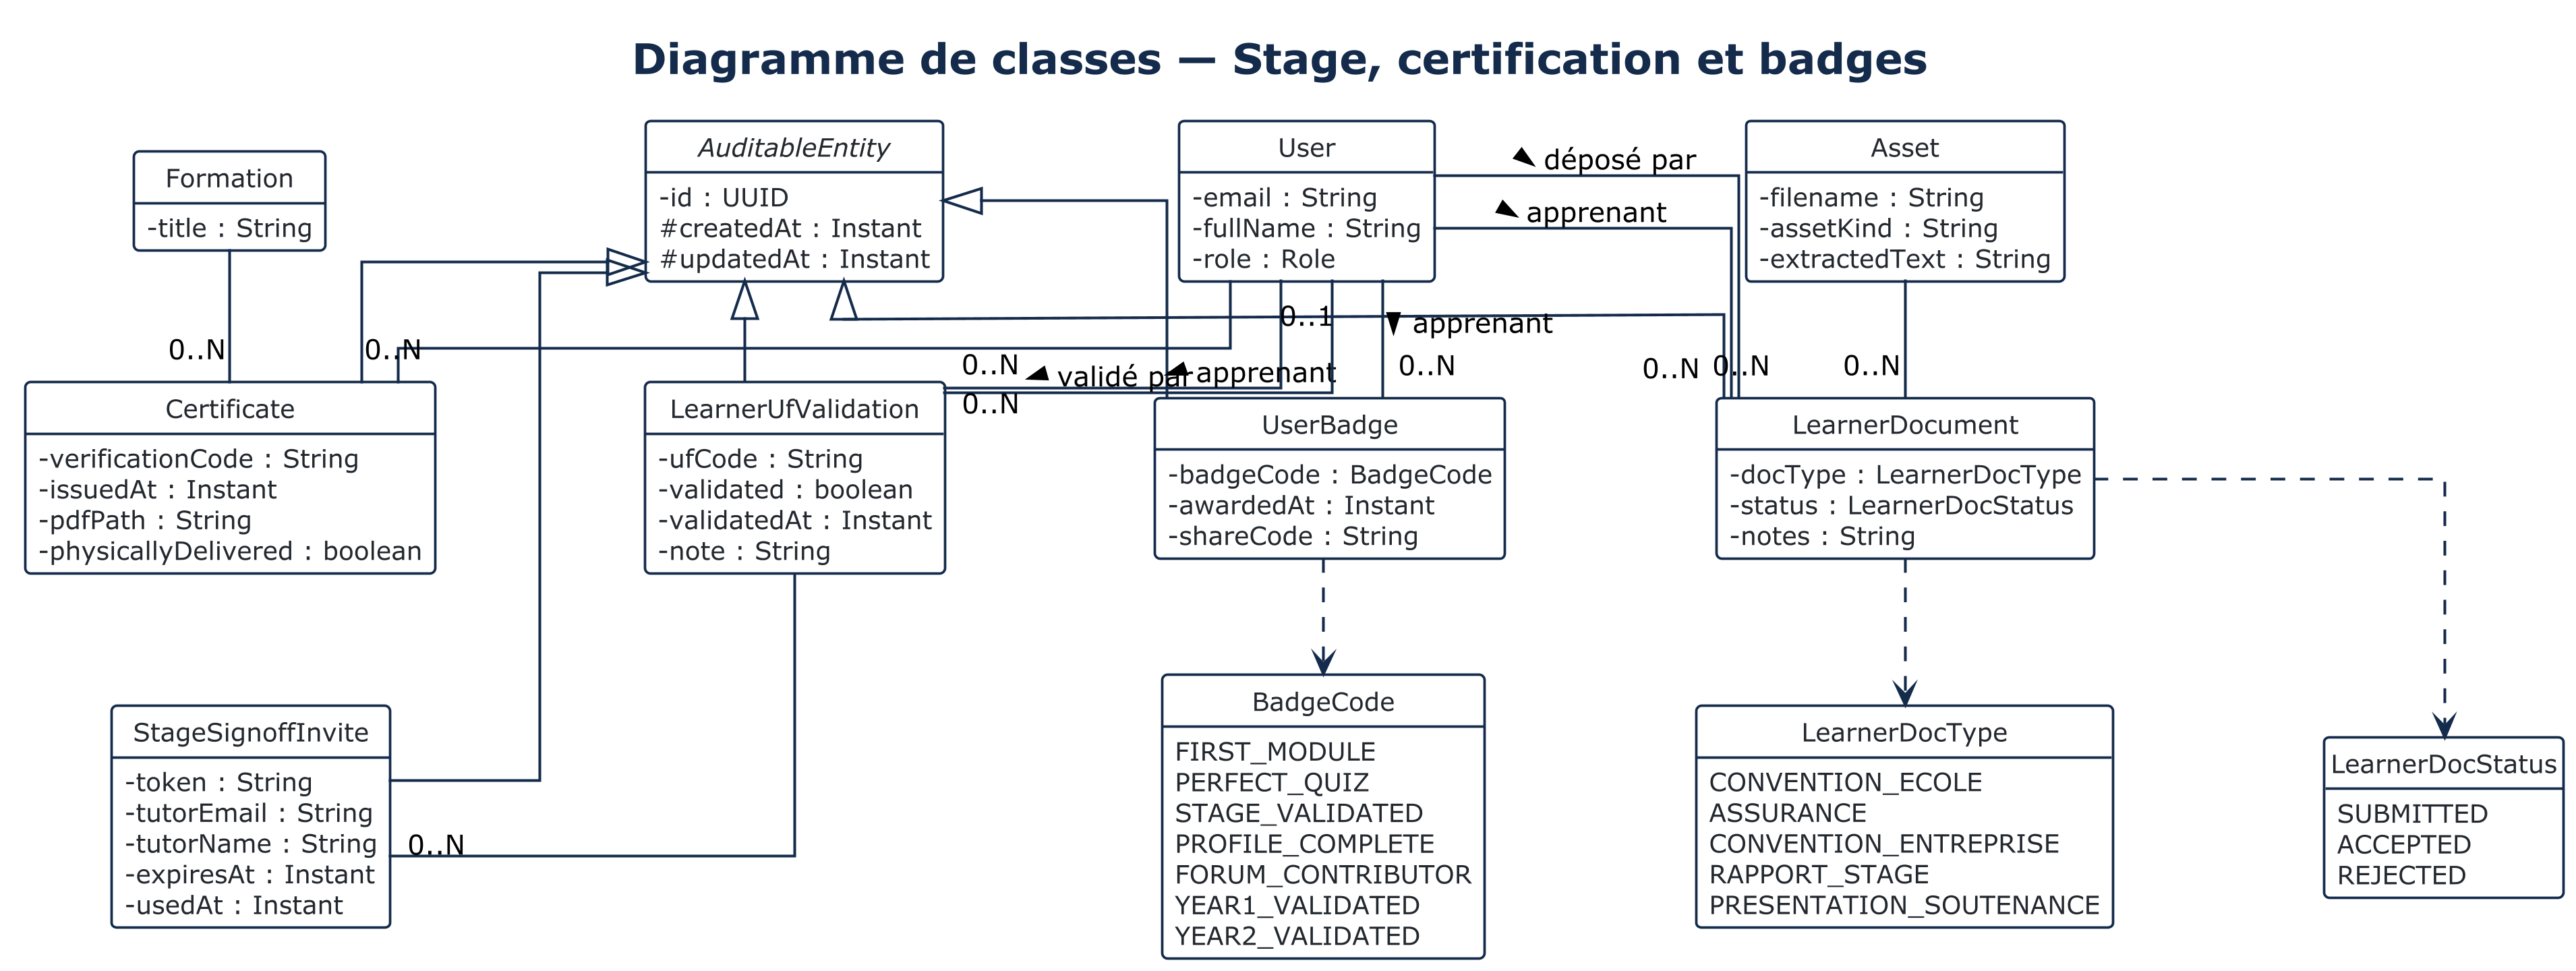
\includegraphics[width=\textwidth,height=0.85\textheight,keepaspectratio]{diagramme_classes_stage_certification.png}
  \caption{Diagramme de classes — stage et certification}
  \label{fig:classes-stage}
\end{figure}

\subsection{Un choix de modélisation délibéré : l'UF comme attribut}

Un choix de conception mérite d'être souligné : l'Unité de Formation (UF)
et l'année du cursus ne sont \emph{pas} modélisées comme des entités
séparées avec leur propre table et clé primaire. Ce sont des attributs
(\texttt{ufCode}, \texttt{ufTitle}, \texttt{yearNumber}) portés directement
par \texttt{ModuleEntity}. Ce choix évite une jointure supplémentaire pour
une notion qui, dans les règles métier réelles, sert uniquement de
\emph{clé de regroupement} (voir \S\ref{sec:progression-uf}) --- il garde
le schéma relationnel simple sans sacrifier la logique de progression par
UF, qui est recalculée dynamiquement à partir de ces attributs plutôt que
stockée redondamment.

\section{Architecture logicielle}

L'application suit une architecture en couches classique
(Figure~\ref{fig:architecture}) : \texttt{Controller} $\rightarrow$
\texttt{Service} $\rightarrow$ \texttt{Repository} $\rightarrow$
\texttt{Entity}, adossée à PostgreSQL pour la persistance et Redis pour les
besoins transverses (limitation de débit, verrous, état éphémère des
tentatives de quiz).

\begin{figure}[H]
  \centering
  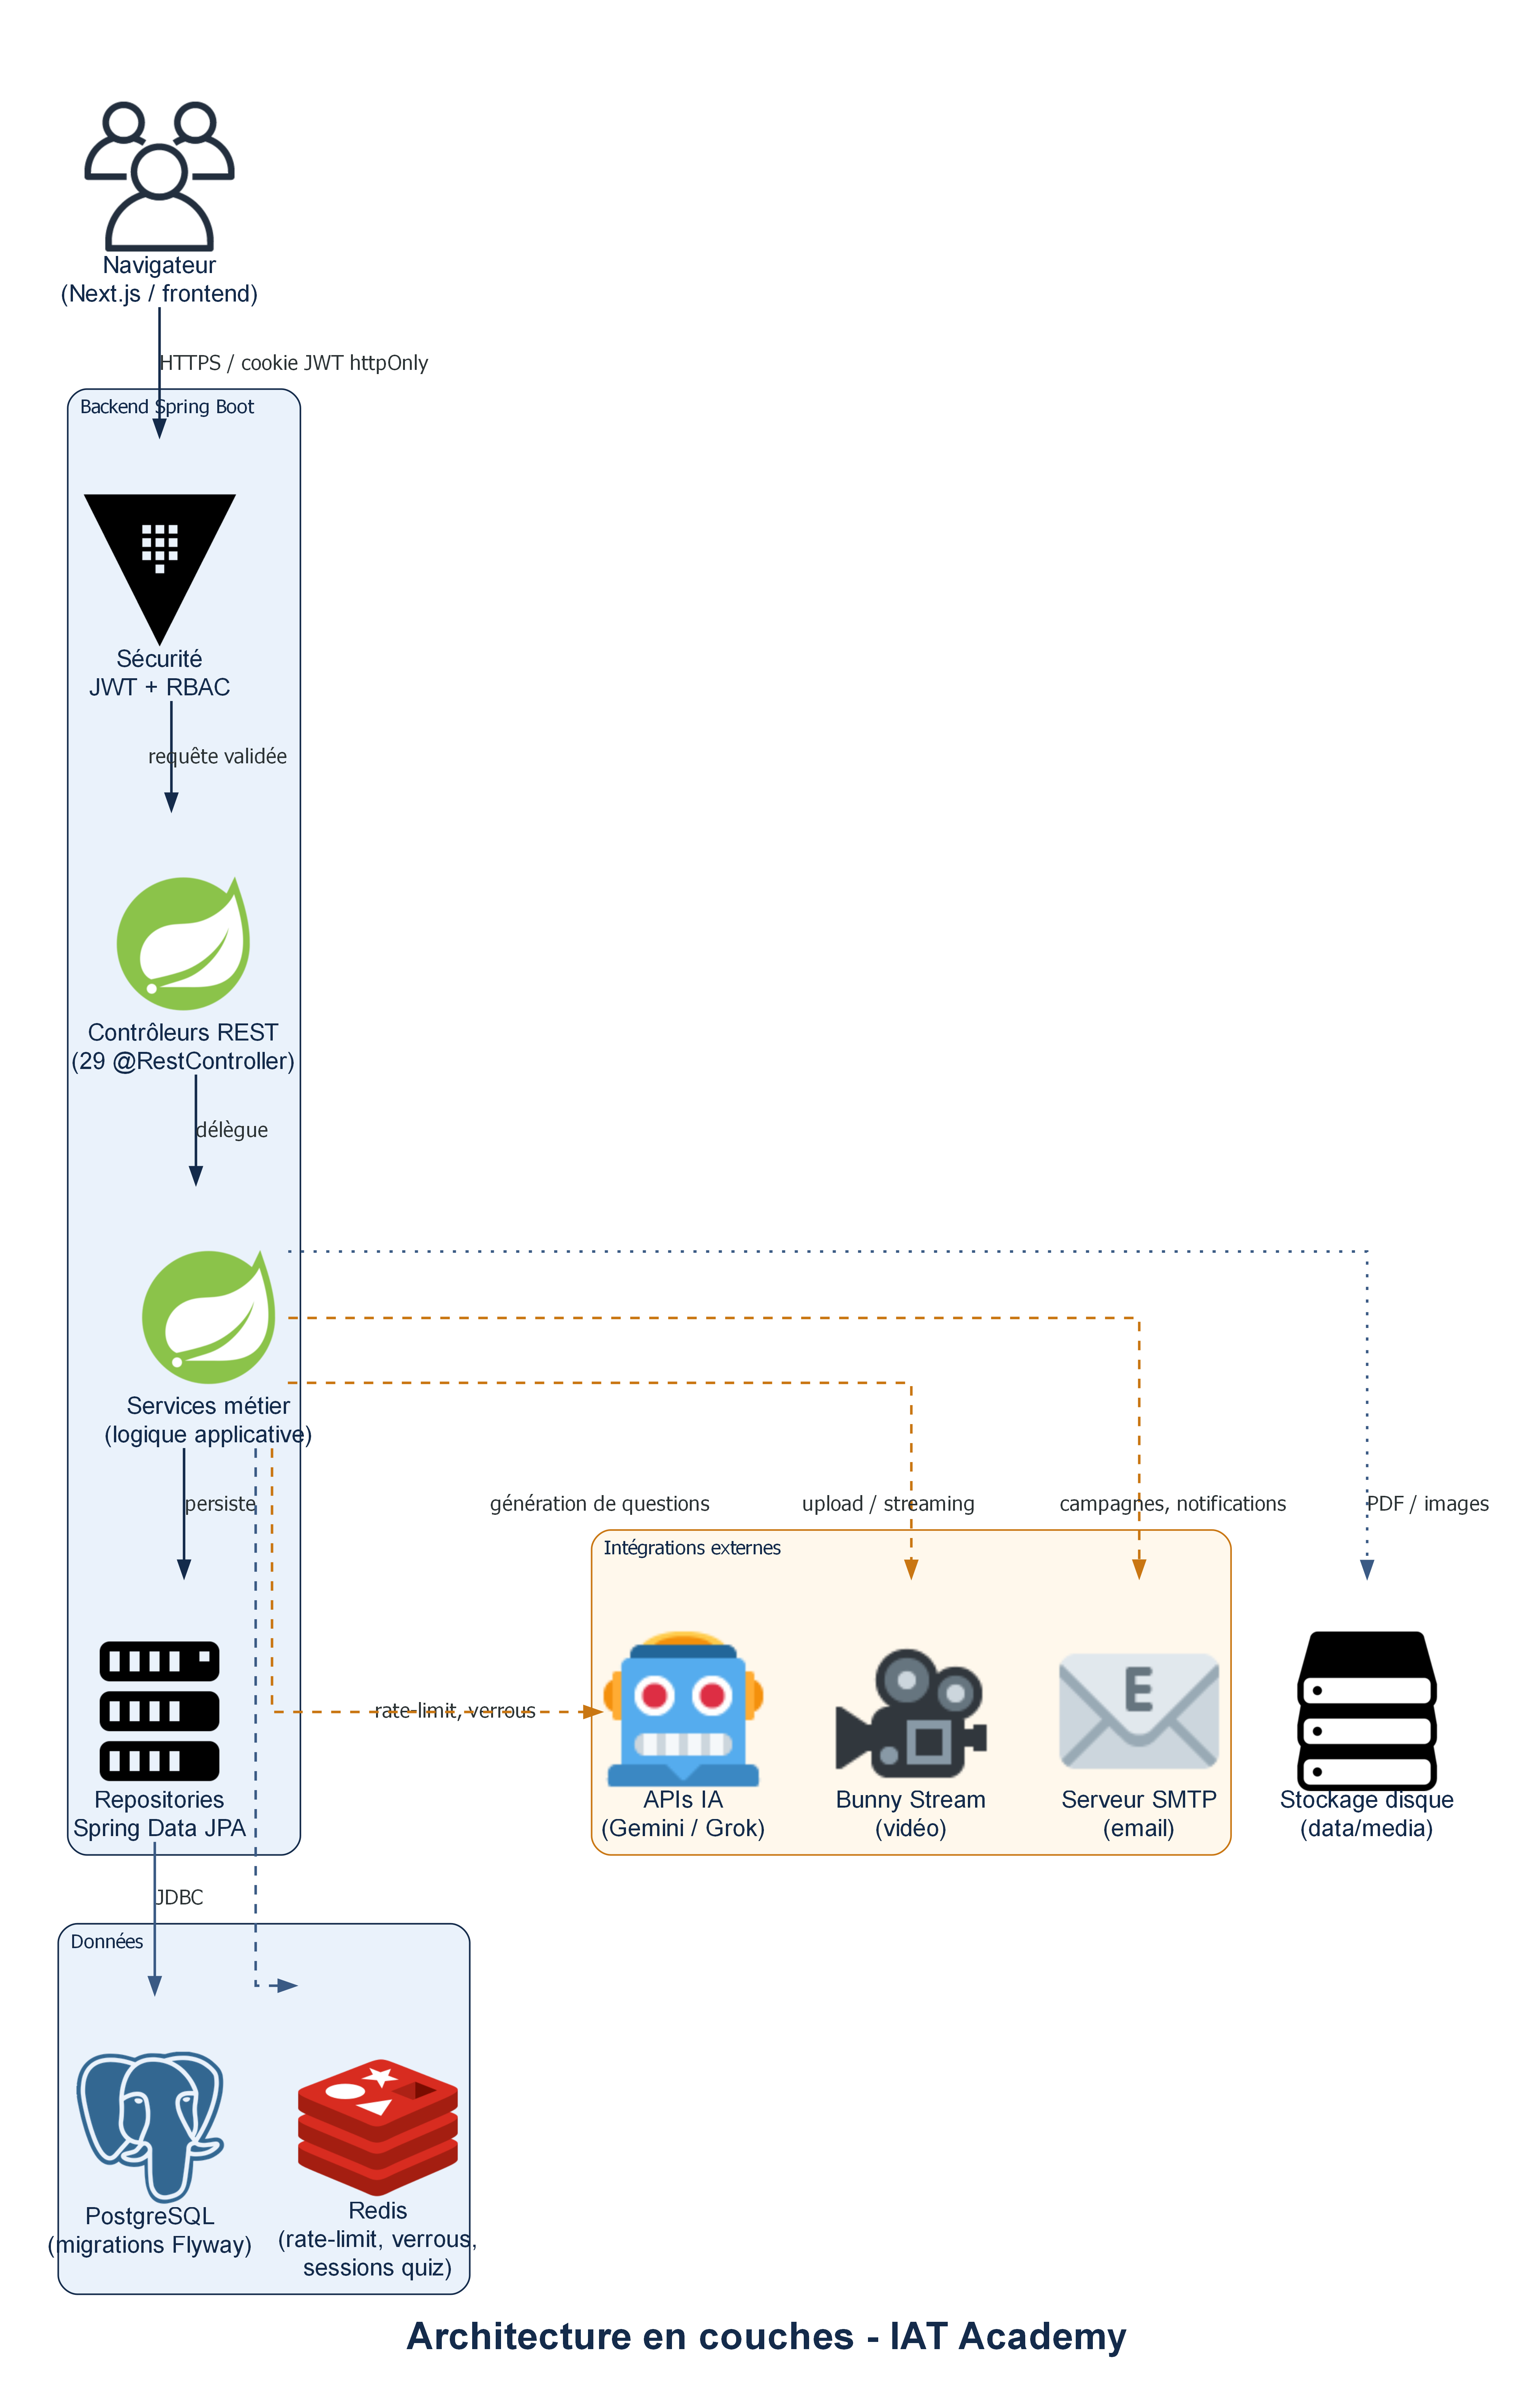
\includegraphics[width=0.75\textwidth,height=0.85\textheight,keepaspectratio]{diagramme_architecture.png}
  \caption{Architecture en couches}
  \label{fig:architecture}
\end{figure}

La règle de conception appliquée de façon constante dans le code est la
suivante : un contrôleur ne fait que du routage HTTP, de la validation
\texttt{@PreAuthorize} et de la traduction requête/réponse ; toute la
logique métier --- y compris les vérifications de propriété de ressource
détaillées au chapitre~\ref{ch:realisation} --- vit dans la couche
service, jamais dans le contrôleur.

\section{Sécurité}

La sécurité de la plateforme ne pouvait pas être traitée comme une simple
case à cocher en fin de développement : dès lors qu'une partie du contenu
--- réponses de quiz, dossiers de stage, échanges de messagerie --- touche
directement à la vie privée et à l'évaluation d'un apprenant mineur ou
jeune majeur, l'authentification et le contrôle d'accès devaient être
pensés comme des contraintes de conception à part entière, et non comme
une couche ajoutée après coup. Cette section détaille les deux piliers sur
lesquels repose cette sécurité : l'authentification, qui répond à la
question \emph{qui êtes-vous ?}, et l'autorisation, qui répond à la
question, en apparence proche mais en réalité bien plus difficile à
garantir correctement, \emph{avez-vous le droit d'agir sur cette
ressource précise ?}

\subsection{Authentification}

L'authentification de la plateforme repose sur un jeton JWT (signé en
HS256) transporté par un cookie \texttt{httpOnly} --- c'est-à-dire un
cookie que le JavaScript exécuté dans le navigateur ne peut ni lire ni
manipuler, ce qui ferme la voie la plus commune d'exfiltration de jeton en
cas de faille de type \emph{cross-site scripting} (XSS) sur le frontend.
Le déroulement complet, depuis la soumission du formulaire de connexion
jusqu'à l'établissement du contexte de sécurité sur chaque requête
suivante, se décompose en quatre étapes. Premièrement,
\texttt{AuthService.login()} authentifie les identifiants soumis par
l'intermédiaire de l'\texttt{AuthenticationManager} de Spring Security,
qui compare le mot de passe fourni au hachage BCrypt stocké en base ---
jamais le mot de passe en clair. Deuxièmement, si l'utilisateur a activé
la double authentification par application TOTP (Google Authenticator ou
équivalent), la réponse renvoyée à ce stade n'est pas encore le cookie de
session final, mais un jeton temporaire valable cinq minutes, qui exige un
second appel explicite à l'endpoint \texttt{/verify-2fa} avant que la
connexion ne soit réellement effective --- une étape supplémentaire
délibérément conçue pour qu'un mot de passe compromis seul ne suffise
jamais à usurper un compte protégé par 2FA. Troisièmement, une fois
l'authentification (simple ou renforcée par 2FA) confirmée,
\texttt{JwtService} construit le jeton définitif, dont le sujet est
l'identifiant de l'utilisateur et dont les revendications embarquent son
adresse email et son rôle applicatif. Quatrièmement, à chaque requête
suivante, \texttt{JwtAuthenticationFilter} --- un filtre Spring exécuté
avant le filtre d'authentification standard du framework --- extrait ce
jeton du cookie, le valide, puis peuple le contexte de sécurité de la
requête courante avant que celle-ci n'atteigne le contrôleur ciblé.

Ce choix architectural a une conséquence directe sur la politique de
session retenue : le backend fonctionne en mode \texttt{STATELESS},
c'est-à-dire qu'aucune session n'est conservée en mémoire côté serveur.
L'intégralité de l'état d'authentification est reconstruite, à chaque
requête, à partir du seul contenu du jeton --- un choix cohérent avec une
architecture où le frontend Next.js est physiquement découplé du backend
Spring Boot, et qui simplifie d'autant la mise à l'échelle horizontale de
l'API si elle devait un jour être répliquée sur plusieurs instances,
puisqu'aucune session partagée n'a besoin d'être synchronisée entre elles.

\subsection{Autorisation}
\label{sec:autorisation}

Savoir \emph{qui} fait la requête ne suffit pas à savoir si cette requête
doit être acceptée : le contrôle d'accès de la plateforme combine, de
façon volontairement distincte, deux niveaux de vérification qui ne
répondent pas à la même question. Le premier niveau est un
\textbf{RBAC déclaratif}, appliqué au moyen de l'annotation
\texttt{@PreAuthorize} posée sur chaque endpoint sensible, et résolu
contre la hiérarchie de rôles \texttt{ROLE\_SUPER\_ADMIN > ROLE\_ADMIN}
présentée au chapitre~\ref{ch:realisation}. Ce niveau répond correctement
à la question \og cet utilisateur a-t-il le \emph{type} de compte requis
pour accéder à cette fonctionnalité ? \fg, mais il est structurellement
incapable de répondre à une seconde question, tout aussi critique dès lors
qu'une ressource appartient nommément à un utilisateur précis : \og cet
utilisateur a-t-il le droit d'accéder à \emph{cette instance précise} de
la ressource, et pas seulement à des ressources de ce type en général ?
\fg. C'est pour répondre à cette seconde question qu'un second niveau, un
\textbf{contrôle de propriété} implémenté au niveau de la couche service,
vient compléter le RBAC pour les ressources intrinsèquement personnelles
--- une conversation de messagerie, une notification, un dossier de stage
--- comme le détaille et l'illustre concrètement le
\S\ref{sec:acces-proprietaire} du chapitre suivant.

\section{Choix technologiques}

Chaque brique technologique retenue pour ce projet répond à une
contrainte identifiée dans les sections précédentes, plutôt qu'à un
simple effet de mode : le Tableau~\ref{tab:stack} met en regard chaque
choix et la justification qui le sous-tend, en particulier pour les
décisions les moins évidentes de prime abord --- pourquoi Redis en plus
d'une base relationnelle déjà présente, ou pourquoi un rendu serveur côté
frontend pour une seule page de la plateforme.

\begin{table}[H]
  \centering
  \caption{Stack technique et justification}
  \label{tab:stack}
  \begin{tabular}{@{}p{3.2cm}p{9cm}@{}}
    \toprule
    Technologie & Justification \\
    \midrule
    Spring Boot 3 / Java 21 & Écosystème mature, sécurité (Spring Security)
      et accès aux données (Spring Data JPA) intégrés, adapté à une
      application métier avec des règles de progression complexes. \\
    PostgreSQL + Flyway & Base relationnelle fiable pour un modèle fortement
      structuré (formations/modules/leçons) ; migrations versionnées
      reproductibles entre environnements. \\
    Redis & Structures de données en mémoire adaptées aux besoins
      transverses à courte durée de vie (compteurs de débit, verrous
      d'édition, état de tentative de quiz) sans alourdir PostgreSQL de
      lectures/écritures fréquentes et volatiles. \\
    JWT + cookie httpOnly & Authentification sans état, compatible avec un
      frontend découplé (Next.js), sans exposer le jeton au JavaScript
      (protection XSS). \\
    Next.js 15 (frontend) & Rendu serveur pour les pages publiques exigeant
      des métadonnées SEO/Open Graph (ex. vérification de certificat, voir
      \S\ref{sec:certificat-linkedin}). \\
    \bottomrule
  \end{tabular}
\end{table}

\section{Conclusion}

Ce chapitre a présenté les cas d'utilisation, le modèle de données, les
choix d'architecture et de sécurité qui structurent IAT Academy. Le
chapitre~\ref{ch:realisation} détaille maintenant comment ces choix se
traduisent dans l'implémentation, en particulier sur les mécanismes qui
dépassent le CRUD simple.

\include{chapitres/ch3_realisation}
\include{chapitres/ch4_tests_deploiement}

\chapter*{Conclusion générale}
\addcontentsline{toc}{chapter}{Conclusion générale}

Ce projet de fin d'études a permis de concevoir et de développer IAT
Academy, une plateforme e-learning complète destinée aux métiers de
l'aviation, de l'accueil et du tourisme, en couvrant l'ensemble du cycle de
vie d'un projet logiciel : analyse des besoins, modélisation d'un domaine
métier de 39 entités, conception d'une architecture en couches robuste,
implémentation d'une API REST sécurisée de 29 contrôleurs, puis validation
par une suite de 138 tests automatisés et une démarche de déploiement
conteneurisé. Au-delà de la couverture fonctionnelle --- catalogue de
cours, système de quiz à quatre portées, gestion de stage, certification
--- ce travail a surtout été l'occasion d'aller au-delà du simple CRUD sur
plusieurs points précis, détaillés au chapitre~\ref{ch:realisation} :
l'intégration résiliente d'un service d'intelligence artificielle
générative avec repli automatique entre deux fournisseurs, la
réconciliation d'état entre correction automatique et correction manuelle
d'un même quiz, une logique de progression pédagogique en cascade jusqu'à
l'éligibilité au certificat, et un contrôle d'accès à granularité fine qui
dépasse le simple contrôle par rôle.

Ce travail n'a pas été mené sans difficultés. La principale d'entre elles a
consisté à traduire des règles métier parfois implicites --- notamment la
distinction entre les UF qui exigent une validation manuelle du Directeur
et celles qui n'en exigent pas, ou encore la coexistence de deux stratégies
de déblocage du contenu selon qu'un apprenant suit son parcours en ligne de
façon autonome ou qu'il appartient à une cohorte encadrée --- en un modèle
de données et une logique applicative à la fois simples et fidèles à la
réalité du terrain. La confrontation régulière avec l'équipe pédagogique
d'IAT Academy a été déterminante pour éviter qu'une simplification
excessive du modèle ne finisse par trahir ces règles. Le chapitre~3 assume
également, en toute transparence, deux limites concrètes identifiées dans
le code existant --- une incohérence dans l'application du contrôle de
propriété au niveau du service de gestion des devoirs, et l'absence d'une
reprise automatique après l'interruption d'une campagne email --- qui
constituent naturellement les premières pistes d'amélioration à court
terme.

À plus long terme, plusieurs évolutions permettraient d'enrichir encore la
plateforme : l'activation complète de la topologie de déploiement déjà
anticipée par la configuration nginx (services API et frontend
conteneurisés aux côtés de PostgreSQL et Redis), la mise en place d'une
intégration continue automatisée pour exécuter la suite de tests à chaque
modification, ou encore l'extension du mécanisme de génération de
questions par intelligence artificielle à d'autres formats pédagogiques.
Au-delà de l'aspect technique, ce stage a été une expérience professionnelle
formatrice à part entière : il a permis de mettre en pratique, sur un projet
réel destiné à des utilisateurs réels, des compétences d'analyse, de
conception et de rigueur technique qui dépassent largement le cadre d'un
exercice académique classique.

% -----------------------------------------------------------------------------
% Bibliographie
% -----------------------------------------------------------------------------
\printbibliography[title={Bibliographie}]

\end{document}
